\documentclass[11pt,a4paper]{article}

\usepackage[spanish]{babel}
\usepackage[math,light]{iwona}
\usepackage[utf8]{inputenc}
\usepackage{amsmath, amsthm}
\usepackage{amsfonts, amssymb, latexsym}
\usepackage{enumerate}
\usepackage[usenames, dvipsnames]{color}
\usepackage{graphics,graphicx, float} %para incluir imágenes y colocarlas
\usepackage{colortbl}
\usepackage{graphicx}
\usepackage{wrapfig}
\usepackage[top=4cm]{geometry}
\usepackage{cite}
\usepackage[official]{eurosym}
\usepackage{cancel}
\usepackage{subfigure}
\usepackage{minted}

\theoremstyle{plain}
\newtheorem{exe}{Ejercicio} % reset theorem numbering for each chapter

\theoremstyle{definition}
\newtheorem{sol}{Solución}

\usepackage[bookmarks=true,
            bookmarksnumbered=false, % true means bookmarks in
                                     % left window are numbered
            bookmarksopen=false,     % true means only level 1
                                     % are displayed.
            colorlinks=true,
            linkcolor=webblue,
            citecolor=red]{hyperref}
\definecolor{webgreen}{rgb}{0, 0.5, 0} % less intense green
\definecolor{webblue}{rgb}{0, 0, 0.5}  % less intense blue
\definecolor{webred}{rgb}{0.5, 0, 0}   % less intense red

\setlength{\parindent}{0pt}
\setlength{\parskip}{1ex plus 0.5ex minus 0.2ex}

\newcommand{\HRule}{\rule{\linewidth}{0.5mm}}

\renewcommand\thesubsection{\alph{subsection}}

\title{\Huge{Visión por Computador} \\ Práctica 3}
\author{Marta Gómez Macías}

\begin{document}
%Cambiar Cuadros por Tablas y lista de...
\renewcommand{\listtablename}{Índice de tablas}
\renewcommand{\tablename}{Tabla}

\maketitle

\tableofcontents

\setcounter{section}{-1}
\section{Opción desarrollada}

Antes de empezar la práctica, aclarar que he escogido la \textbf{opción 1}.

\section{Estimación de la matriz cámara a partir de puntos 3D y sus proyecciones 2D.}

\subsection{Generar una matriz de cámara finita con valores aleatorios en $[0,1]$.}

Para que una matriz defina una cámara debe cumplir las siguientes condiciones:

\begin{enumerate}[---]
\item Ser una matriz $3 \times 4$.

\begin{displaymath}
P_{3\times 4} = [M_{3\times 3} | p_{3 \times 1}]
\end{displaymath}

\item Que el determinante de la submatriz $M_{3 \times 3}$ sea distinto de cero.

\begin{displaymath}
det(M) \neq 0
\end{displaymath}

\end{enumerate}

En la función implementada, genero una matriz $3 \times 4$ aleatoria inicial, si no cumple la condición de que su determinante de $M$ sea distinto de cero, vuelvo a generar otra matriz aleatoria, hasta conseguir una que cumpla la condición. La función \texttt{random.rand} de \textit{Numpy} nos asegura números aleatorios en el rango $[0,1]$.

\begin{minted}[frame=lines, label={Generación de una cámara}]{python}
def genera_camara_finita():
    P = np.random.rand(3,4)
    while np.linalg.det(P[:3,:3]) == 0:
        P = np.random.rand(3,4)
    P=P/P[-1,-1]
    return P
\end{minted}

\subsection{Generar puntos 3D en dos planos distintos ortogonales.}

Para que los puntos generados cumplan la condición de pertenecer a dos planos distintos ortogonales deben tener la siguiente forma:

\begin{displaymath}
\{(0,x_1,x_2)\;y\;(x_2,x_1,0), \qquad\ donde\;x_1 = [0.1,0.1,1]\;y\;x_2=[0.1,0.1,1]\}
\end{displaymath}

es decir, tanto $x_1$ como $x_2$ son todos los números desde el $0,1$ hasta el $1$ en intervalos de $0,1$: $0.1, 0.2, 0.3, \cdots 1$.

\begin{minted}[frame=lines, label={Generación de puntos 3D}]{python}
def genera_puntos_planos_ortogonales_distintos():
    # posibles valores para x1 y x2
    x1 = x2 = np.arange(start=0.1,stop=1,step=0.1,dtype=np.float32)
    # generamos un conjunto de puntos con todas las combinaciones de (x1,x2)
    conjunto = np.concatenate(np.array(np.meshgrid(x1,x2)).T)
    # y le añadimos una columna de ceros al principio
    zeros_vector = np.zeros(conjunto.shape[0])
    conjunto1 = np.hstack((zeros_vector[..., None], conjunto))
    # y otra al final
    conjunto2 = np.hstack((conjunto, zeros_vector[...,None]))

    return np.concatenate((conjunto1, conjunto2))
\end{minted}

\subsection{Proyectar los puntos 3D generados con la cámara $P$ simulada.}

Para calcular la proyección de un 3D con una cámara $P$ debemos multiplicar la cámara por el punto:

\begin{displaymath}
x_{3 \times 1} = P_{3 \times 4} \cdot X_{4 \times 1}
\end{displaymath}

Debemos convertir el punto 3D $X$ a coordenadas homogéneas (añadiéndole un $1$ como última coordenada) para poder multiplicarlo por la matriz de la cámara. Una vez hecha la multiplicación, obtenemos un vector $x$ con tres elementos, pero un punto 2D sólo tiene dos coordenadas, por lo que debemos eliminar el último elemento del vector:

\begin{displaymath}
x_x = \frac{x_x}{x_z} \qquad\ x_y = \frac{x_y}{x_z}
\end{displaymath}

\begin{minted}[frame=lines, label={Proyección de los puntos 3D con P}]{python}
camera_projection = lambda x, P: P.dot(np.hstack((x,[1])))

def proyecta_puntos_en_plano(camara, puntos):
    # definimos el array en el que guardaremos las coordenadas píxel de los puntos
    conjunto = np.zeros(puntos.shape)
    # iteramos sobre el array de puntos del mundo para proyectar los puntos
    for i in range(puntos.shape[0]):
        conjunto[i] = camera_projection(x=puntos[i], P=camara)

    # calculamos las coordenadas píxel diviendo la coordenada x e y por la coord z
    coords_pixel = np.zeros((puntos.shape[0], 2))
    for i in range(puntos.shape[0]):
        z = conjunto[i,2]
        coords_pixel[i,0] = conjunto[i,0]/z
        coords_pixel[i,1] = conjunto[i,1]/z

    return coords_pixel
\end{minted}

\subsection{Implementar el algoritmo DLT.}

Para realizar este apartado me he basado en \cite{mvg} y \cite{forelas}.

Dados unos puntos 3D, $X$ y sus proyecciones en 2D, $x$, queremos estimar la matriz de la cámara $P$.

\begin{displaymath}
x_i = P \cdot X_i \qquad\ i = 1, \ldots, N
\end{displaymath}

Cada punto tiene $x$ tiene 3 ecuaciones distintas:

\begin{displaymath}
\left[ 
    \begin{array}{ccc}
    0^T & -X_i^T & y_i\cdot X_i^T \\
    X_i^T & 0^T & -x_i\cdot X_i^T \\
    -y_i \cdot X_i^T & x_i \cdot X_i^T & 0^T
    \end{array} \right] \left( \begin{array}{c}
    P^1 \\
    P^2 \\
    P^3
    \end{array} \right) = 0
\end{displaymath}

donde cada $P^{iT}$ es un vector de 4 elementos que contiene la $i$-ésima fila de $P$. Debido a que estas tres ecuaciones son linealmente dependientes, podemos quedarnos únicamente con las dos primeras:

\begin{displaymath}
\underbrace{\left[ 
    \begin{array}{ccc}
    X_i^T & 0^T & -x_i\cdot X_i^T\\
    0^T & X_i^T & -y_i\cdot X_i^T
    \end{array} \right]}_{M_i} \left( \begin{array}{c}
    P^1 \\
    P^2 \\
    P^3 
    \end{array} \right) = 0
\end{displaymath}

Para cada punto calcularemos su matriz $M_i$ y haremos una matriz $M$ con un total de $2N$ filas. Como mínimo, $N \geq 6$, ya que la matriz $P$ tiene 12 elementos y (ignorando la escala) 11 grados de libertad, por lo que debemos tener 11 ecuaciones para resolver $P$, debido a que cada punto nos da dos ecuaciones, necesitamos como mínimo $5,5$ puntos.

Una vez hayamos obtenido la matriz $M$, pasaremos a calcular su \textbf{descomposición en valores singulares}:

\begin{displaymath}
SVD(M) = USV^T
\end{displaymath}

La matriz $S$ contiene los autovalores de $M$ y $V$, los autovectores. Nuestra matriz $P$ será el autovector con un menor autovalor, es decir, la última columna de la matriz $V^T$.

\subsubsection{Normalización}

Para evitar que los valores de la matriz $M$ tengan una alta varianza, debemos normalizar los puntos antes de calcular la matriz. Para normalizar los puntos, aplicamos a cada punto la siguiente matriz de normalización:

\begin{enumerate}[---]
\item Si el punto es 2D:

\begin{displaymath}
T = \left[ \begin{array}{ccc}
                s & 0 & m_x \\
                0 & s & m_y \\
                0 & 0 & 1
              \end{array} \right]
\end{displaymath}
              
\item Si el punto es 3D:

\begin{displaymath}
U = \left[ \begin{array}{cccc}
                s & 0 & 0 & m_x \\
                0 & s & 0 & m_y \\
                0 & 0 & s & m_z \\
                0 & 0 & 0 & 1
              \end{array} \right]
\end{displaymath}
\end{enumerate}

Donde $s$ es la desviación media de $M$ y $m$ la media de las distintas coordenadas $x$, $y$ y $z$. Estas matrices se deben guardar, ya que se utilizan para \textbf{deshacer la normalización} al final del algoritmo:

\begin{displaymath}
P = T^{-1}\tilde{P}U
\end{displaymath}

\begin{minted}[frame=lines, label={Algoritmo DLT}]{python}
def norm_points(points):
    media = np.mean(a=points, axis=0)
    desv_std = np.std(a=points)
    dims = points.shape[1] # para saber si estamos en 3d o 2d
    if dims==2:
        Tr = np.array([[desv_std, 0, media[0]],[0, desv_std, media[1]],[0,0,1]])
    else:
        Tr = np.array([[desv_std, 0, 0, media[0]], [0, desv_std, 0, media[1]], 
            [0, 0, desv_std, media[2]], [0,0,0,1]])

    Tr = np.linalg.inv(a=Tr)
    x = np.dot(Tr, np.concatenate((points.T, np.ones((1,points.shape[0])))))
    x = x[0:dims,:].T
    return Tr, x

def DLT(X, x):
    n = x.shape[0] # numero de puntos
    # M tendrá, para cada punto, 2 filas y 12 columnas. Sólo usamos 2 filas 
    # ya que las tres ecuaciones de la matriz M son
    # linealmente dependientes.
    M = np.zeros(shape=(2*n, 12))
    z = np.zeros(shape=(4))
    # normalizamos los puntos
    tr, xn = norm_points(x)
    Tr, Xn = norm_points(X)
    # calculamos la matriz M
    for i in range(0,2*n,2):
        j = int(i/2)
        M[i] = np.concatenate((Xn[j], [1], z, -xn[j,0]*Xn[j], [-xn[j,0]]))
        M[i+1] = np.concatenate((z, Xn[j], [1], -xn[j,1]*Xn[j], [-xn[j,1]]))
    # calculamos sus valores propios
    U,S,V = np.linalg.svd(a=M)
    # La última fila de V contiene el autovector con menor autovalor (S).
    P = (V[-1]/V[-1,-1]).reshape(3,4)
    # deshacemos la normalización
    P = np.dot(np.dot(np.linalg.pinv(tr), P), Tr)
    P = P/P[-1,-1]
    return P
\end{minted}

La cámara generada aleatoriamente fue:

\begin{displaymath}
\left[
\begin{matrix}
1.96197176 & 0.53239387 & 0.58397881 & 0.41685435 \\
1.98123967 & 1.03400467 & 0.08051371 & 2.29137397 \\
0.11581623 & 2.23907194 & 2.81127508 & 1
\end{matrix}
\right]
\end{displaymath}

Mientras que la cámara estimada por nuestro algoritmo fue:

\begin{displaymath}
\left[
\begin{matrix}    
1.96197176 & 0.53239387 & 0.58397881 & 0.41685435 \\
1.98123967 & 1.03400467 & 0.08051371 & 2.29137397 \\
0.11581623 & 2.23907194 & 2.81127508 & 1
\end{matrix}
\right]
\end{displaymath}

Las cámaras obtenidas son iguales. Por tanto, podemos concluir que hemos realizado una estimación correcta.

\subsection{Calcular el error de la estimación usando la norma de Frobenius.}

Para calcular el error de la cámara estimada he calculado su ``distancia'' a la cámara real:

\begin{displaymath}
error = \sqrt{\sum_{i,j} abs(P^{real}_{ij} - P^{estimada}_{ij})^2}
\end{displaymath}

La norma de Frobenius está implementada en numpy en la función \href{https://docs.scipy.org/doc/numpy/reference/generated/numpy.linalg.norm.html}{\texttt{linalg.norm}}, usando el parámetro \texttt{ord=None}.

\begin{minted}[frame=lines, label={Estimación del error de la cámara estimada}]{python}
def estima_error(orig, estimada):
    return np.linalg.norm(x=(orig - estimada), ord=None)
\end{minted}

El error obtenido en la cámara estimada fue igual a $3.73946539938 \cdot 10^{-14}$. Como dije antes, ambas cámaras son prácticamente iguales ya que para encontrar diferencias entre ambas tenemos que irnos a la decimoquinta cifra decimal.

\subsection{Mostrar en una única imagen los puntos 3D proyectados con la cámara estimada y la cámara simulada.}

En azul muestro los puntos proyectados con la cámara simulada y en rojo, los de la cámara estimada.

\begin{minted}[frame=lines, label={Dibujando los puntos 3D proyectados por ambas cámaras}]{python}
def draw_points(real_points, estimated_points):
    # creamos una imagen vacía
    img = np.ones(shape=(200,100,3), dtype=np.uint8)
    rp = np.array(100*real_points, dtype=np.int32)
    ep = np.array(100*estimated_points, dtype=np.int32)
    # pintamos los distintos puntos
    for i in range(real_points.shape[0]):
        cv2.circle(img=img, radius= 1, center=(rp[i,0], rp[i,1]), \
                   color=(255,0,0), thickness=-1)
        cv2.circle(img=img, radius=1, center=(ep[i, 0], ep[i, 1]), \
                   color=(0, 0, 255), thickness=-1)
    mostrar(img)
\end{minted}

\begin{figure}[!h]
    \centering
    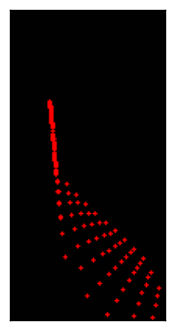
\includegraphics[width=0.2\textwidth]{img1}
    \caption{Resultado de la función \texttt{draw\_points}}
    \label{drawpoints}
\end{figure}

El resultado de esta función se aprecia en la \hyperref[drawpoints]{Figura \ref*{drawpoints}}. En la imagen sólo vemos puntos rojos ya al truncar a entero los puntos proyectados con ambas cámaras obtenemos las mismas coordenadas. Por tanto, los puntos proyectados por la cámara estimada se pintan encima de los puntos estimados por la cámara simulada, obteniendo este resultado. Esta imagen es la prueba de que la cámara estimada obtenida es una buena estimación de la cámara original.

\section{Calibración de la cámara usando homografías}

Para realizar este apartado me he basado en \cite{cal}.

\subsection{Leer las imágenes chessboard, determinar las válidas para calibrar una cámara, calcular sus esquinas y pintarlas}

Este apartado se divide en tres partes:

\begin{enumerate}
\item Leer las imágenes \textit{chessboard} y determinar las que son válidas para calibrar una cámara. Para ello, leeremos todas las imágenes y llamaremos a la función \texttt{findChessboardCorners} y comprobaremos el valor booleano devuelto por la función. Si es verdadero, la imagen es válida para calibrar una cámara.

Para poder saber qué punto del mundo corresponde a cada esquina encontrada, definimos un sistema de coordenadas cuyo centro se encuentra en el tablero. El punto $(0,0)$ se encontraría en la esquina superior izquierda. Así, tenemos definidas de forma sencilla unas correspondencias 2D - 3D que más adelante nos ayudarán a calibrar la cámara.

\item Calcular las esquinas de las imágenes. En este caso, también usamos la función \texttt{findChessboardConers} aunque esta vez nos centramos en las esquinas calculadas por la misma. Para refinar estas esquinas encontradas, usaremos la función \texttt{cornerSubPix}.

\item Pintarlas sobre las mismas. Este último paso lo realizaremos llamando a la función \texttt{drawChessboardCorners}. La imagen sobre la que pintamos las esquinas debe ser una copia de la original, ya que si no ésta se verá modificada.
\end{enumerate}

\begin{minted}[frame=lines, label={Imágenes chessboard}]{python}
def find_valid_imgs(path="chessboard/Image", n_imgs=25, format=".tif", 
                    pat_size=(13,12)):
    valid_imgs = []
    for i in range(n_imgs):
        imgpath = path+str(i+1)+format
        img = cv2.imread(imgpath)
        gray = cv2.cvtColor(src=img, code=cv2.COLOR_BGR2GRAY)
        # encontrar los chess board corner
        retval, corners = cv2.findChessboardCorners(image=gray, patternSize=pat_size,
                            flags=(cv2.CALIB_CB_NORMALIZE_IMAGE +
                                    cv2.CALIB_CB_ADAPTIVE_THRESH
                                    + cv2.CALIB_CB_FAST_CHECK))
        if retval:
            valid_imgs.append(img)

    return valid_imgs

def find_and_draw_chessboard_corners(valid_images, pat_size=(13,12)):
    imgpoints = [] # puntos 2D de la imagen
    objpoints = [] # puntos 3D del mundo real. Tomando como centro del mundo el tablero.
    objp = np.zeros((pat_size[0]*pat_size[1],3),np.float32)
    objp[:,:2] = np.mgrid[0:pat_size[0], 0:pat_size[1]].T.reshape(-1,2)
    objp = objp.reshape(-1,1,3)
    gray_shape = 0

    for img in valid_images:
        gray = cv2.cvtColor(src=img, code=cv2.COLOR_BGR2GRAY)
        gray_shape = gray.shape

        # encontrar los chess board corner
        retval, corners = cv2.findChessboardCorners(image=gray, patternSize=pat_size,
                                flags=(cv2.CALIB_CB_NORMALIZE_IMAGE+
                                        cv2.CALIB_CB_ADAPTIVE_THRESH
                                        +cv2.CALIB_CB_FAST_CHECK))
        # si hemos encontrado, pasamos a refinarlos
        if retval:
            # cada llamada a esta función da un número de puntos entre 0 y 
            # patsize[1]*patsize[0]. Por tanto, nos tendremos que quedar con 
            # los corners2.shape[0] primeros puntos del mundo objp
            corners2 = cv2.cornerSubPix(image=gray, corners=corners, 
                    winSize=(11,11), zeroZone=(-1,-1),
                    criteria=(cv2.TERM_CRITERIA_EPS + 
                        cv2.TERM_CRITERIA_MAX_ITER, 30, 0.001))
            imgpoints.append(corners2)
            objpoints.append(objp)
            # mostramos los corner encontrados
            imgcorners = img.copy()
            imgdraw = cv2.drawChessboardCorners(image=imgcorners, 
                        patternSize=pat_size, corners=corners2,
                        patternWasFound=retval)
            mostrar(imgdraw)

    return imgpoints, objpoints, gray_shape
\end{minted}

\begin{figure}[!h]
    \mbox{
        \subfigure[Primera imagen válida con las esquinas encontradas]{
            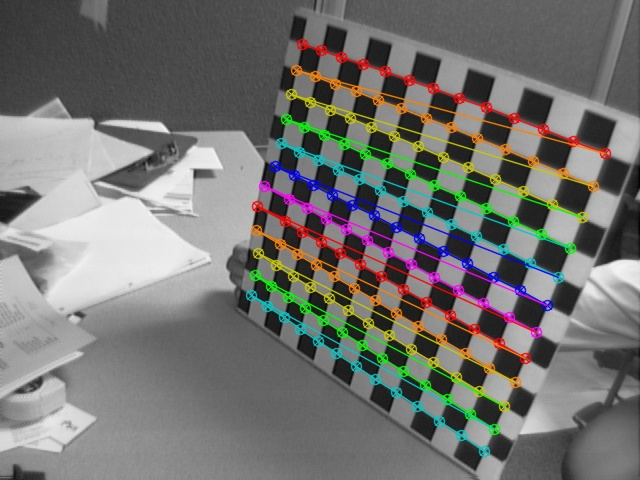
\includegraphics[width=0.5\textwidth]{img2}
            \label{img2}
        }
        \subfigure[Segunda imagen válida con las esquinas encontradas]{
            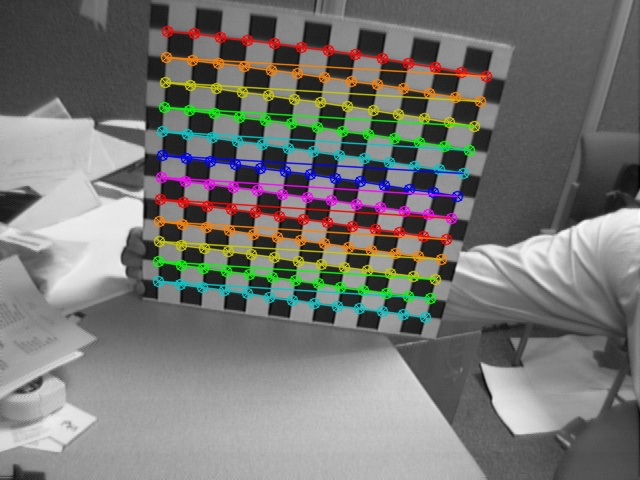
\includegraphics[width=0.5\textwidth]{img3}
            \label{img3}
        }
    }
    \mbox{
        \subfigure[Tercera imagen válida con las esquinas encontradas]{
            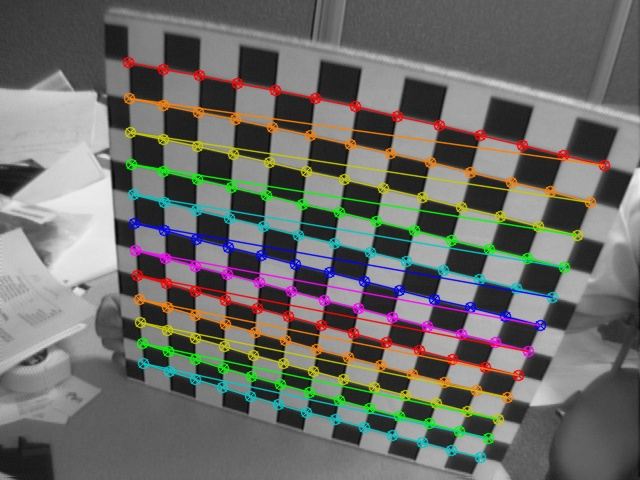
\includegraphics[width=0.5\textwidth]{img4}
            \label{img4}
        }
        \subfigure[Cuarta imagen válida con las esquinas encontradas]{
            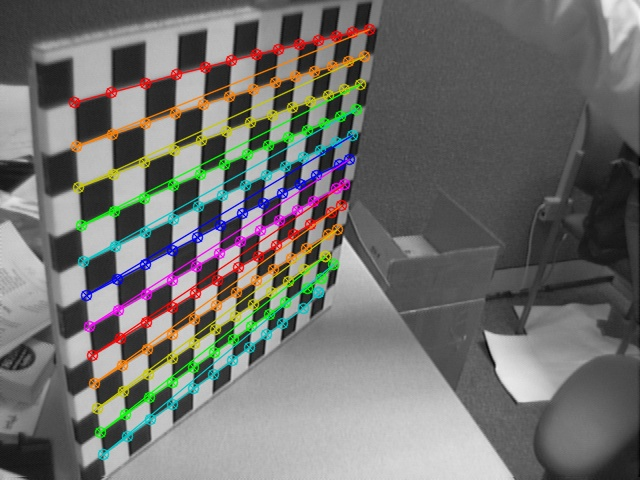
\includegraphics[width=0.5\textwidth]{img5}
            \label{img5}
        }
    }
    \caption{Imágenes válidas con las esquinas encontradas}
    \label{chessboard}
\end{figure}

En la \hyperref[chessboard]{Figura \ref*{chessboard}} vemos los resultados obtenidos por la función desarrollada. Obtenemos un resultado muy bueno: las esquinas obtenidas coinciden con las esquinas del tablero y hemos conseguido un patrón del tablero completo. Además, hemos obtenido cuatro imágenes diferentes, lo cual es suficiente para realizar la calibración.

\subsection{Calcular los parámetros intrínsecos y extrínsecos de la cámara para cada imagen.}

\subsubsection{Sin tener en cuenta la distorsión.}

En este caso, simplemente calibramos la cámara con los puntos encontrados. Para ello, llamamos a la función \texttt{calibrateCamera} pasándole los puntos del mundo 3D definidos por nosotros en el apartado anterior y sus correspondientes puntos 2D calculados.

\begin{minted}[frame=lines, label={calibrando la cámara}]{python}
def calibrate(objpoints, imgpoints, pic_shape):
    ret, mtx, dist, rvecs, tvecs = cv2.calibrateCamera(objectPoints=objpoints, 
                                    imagePoints=imgpoints,
                                    imageSize=pic_shape, cameraMatrix=None, 
                                    distCoeffs=None)

    return mtx, dist, rvecs, tvecs
\end{minted}

El error de reproyección que calculó \textit{OpenCV} para este caso fue de $1.2530441330883588$.

\subsubsection{Teniendo en cuenta la distorsión de las imágenes.}

En este caso, tendremos que corregir la distorsión de las mismas usando la función \texttt{undistort} y la función \texttt{getOptimalNewMatrixCamera} para calcular el parámetro \texttt{newCameraMatrix}.

\begin{minted}[frame=lines, label={calibrando la cámara sin distorsión}]{python}
def calibrate_undistort(valid_images, mtx, dist, pic_shape):
    valid_und_img = []
    # calculamos la camera matrix óptima
    newmtx, roi = cv2.getOptimalNewCameraMatrix(cameraMatrix=mtx, distCoeffs=dist, 
                            imageSize=pic_shape, alpha=1)
    # leemos todas las imágenes de la lista img_index, calculamos 
    # la imagen sin distorsión
    for img in valid_images:
        dst = cv2.undistort(src=img, cameraMatrix=mtx, distCoeffs=dist, 
                            newCameraMatrix=newmtx)
        valid_und_img.append(dst)
        mostrar(dst)
    
    return valid_und_img
\end{minted}

\begin{figure}[!h]
    \mbox{
        \subfigure[Primera imagen válida sin distorsión]{
            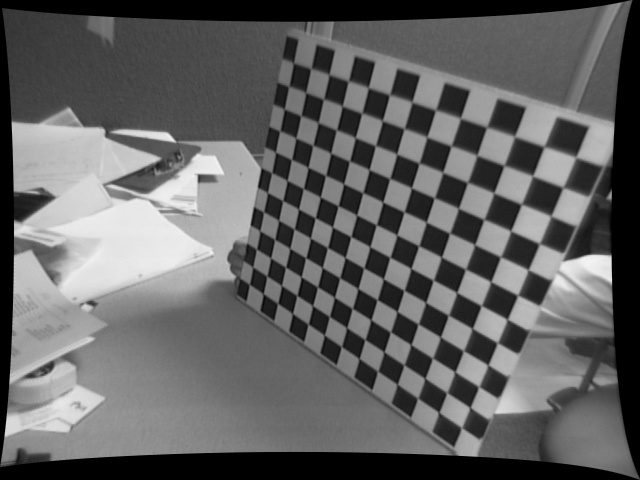
\includegraphics[width=0.5\textwidth]{img6}
            \label{img6}
        }
        \subfigure[Segunda imagen válida sin distorsión]{
            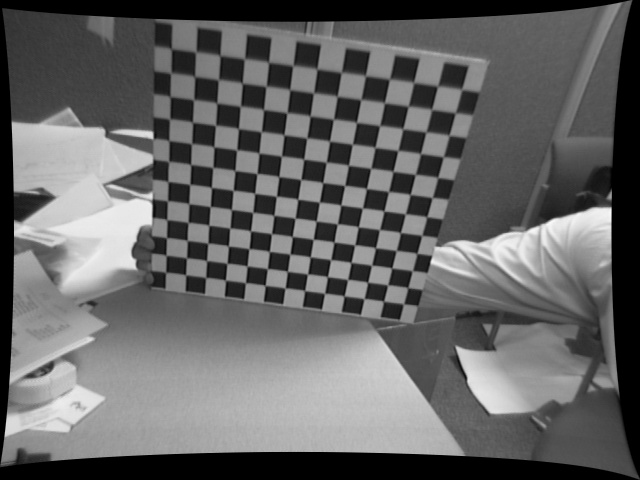
\includegraphics[width=0.5\textwidth]{img7}
            \label{img7}
        }
    }
    \mbox{
        \subfigure[Tercera imagen válida sin distorsión]{
            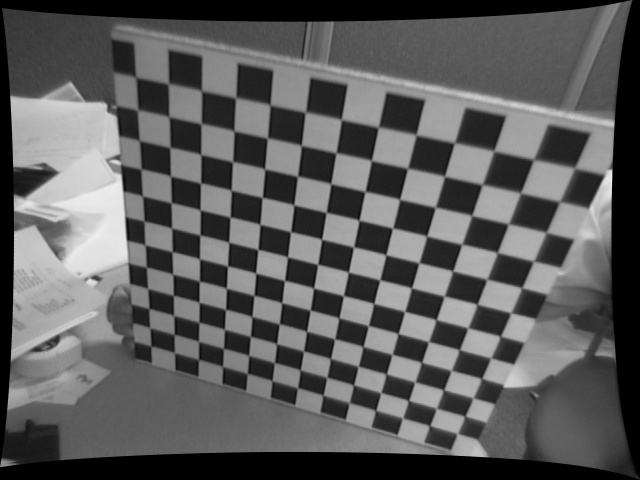
\includegraphics[width=0.5\textwidth]{img8}
            \label{img8}
        }
        \subfigure[Cuarta imagen válida sin distorsión]{
            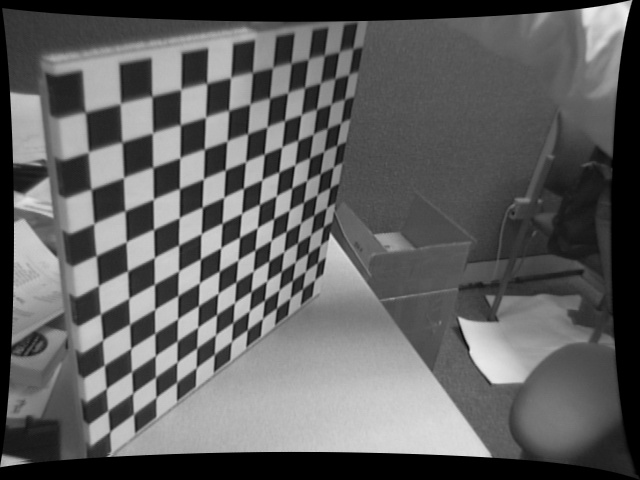
\includegraphics[width=0.5\textwidth]{img9}
            \label{img9}
        }
    }
    \caption{Imágenes válidas sin distorsión}
    \label{undistort}
\end{figure}

En la \hyperref[undistort]{Figura \ref*{undistort}} vemos las imágenes válidas encontradas anteriormente, con la distorsión eliminada. En este caso, creo que las imágenes tenían sobre todo \textbf{distorsión radial}, ya que las correcciones que ha hecho OpenCV son de tipo radial: el centro de la foto se mantiene igual y sólo se corrigen deformaciones en los extremos.

\begin{figure}[!h]
    \centering
    \mbox{
        \subfigure[Primera imagen válida sin distorsión con las esquinas encontradas]{
            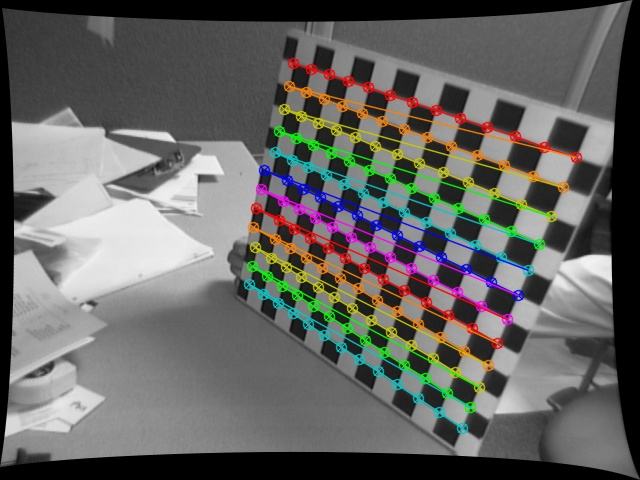
\includegraphics[width=0.5\textwidth]{img10}
            \label{img10}
        }
        \subfigure[Segunda imagen válida sin distorsión con las esquinas encontradas]{
            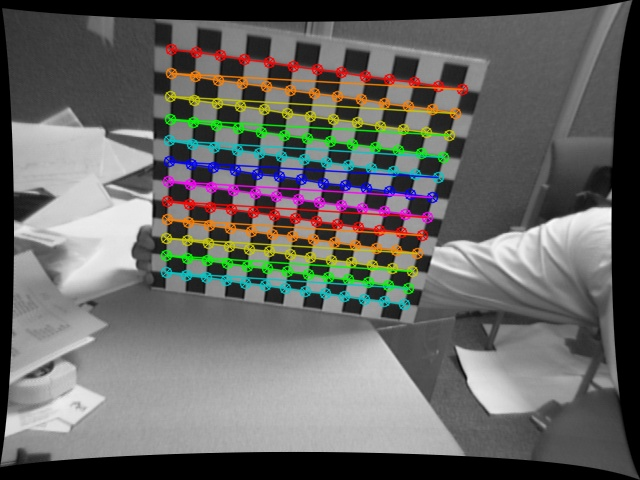
\includegraphics[width=0.5\textwidth]{img11}
            \label{img11}
        }
    }
    \subfigure[Tercera imagen válida sin distorsión con las esquinas encontradas]{
        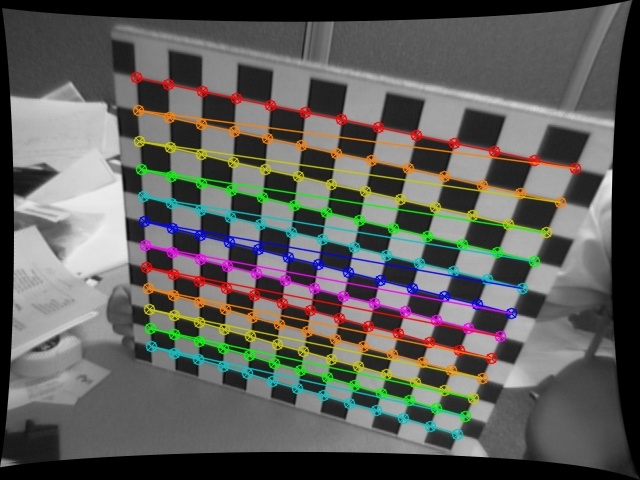
\includegraphics[width=0.5\textwidth]{img12}
        \label{img12}
    }
    \caption{Imágenes válidas sin distorsión con las esquinas encontradas}
    \label{undistortcab}
\end{figure}

En la \hyperref[undistortcab]{Figura \ref*{undistortcab}} vemos las esquinas \textit{chessboard} encontradas en las imágenes sin distorsión. La estimación de la cámara se ha realizado correctamente, ya que como mínimo necesitamos $N \geq 3$ para realizar la calibración. El error de reproyección obtenido en este caso al calibrar la cámara fue de $0.6982332859239562$  Como vemos, el error obtenido al eliminar la distorsión de las imágenes ha sido mucho menor. Por tanto, podemos concluir que la distorsión ha jugado un papel decisivo.

\newpage
A continuación muestro los parámetros obtenidos en el caso con distorsión y el caso sin distorsión:

\begin{center}
    {\LARGE \textbf{Cámara}}
\end{center}
\begin{minipage}{0.5\textwidth}
\begin{center}
{\Large \textbf{Con distorsión}}
\end{center}
\begin{displaymath}
\left[
\begin{matrix}
655.60434 &   0 &         301.47609 \\
  0 &         661.07442 & 229.11322 \\
  0 &           0 &           1   
\end{matrix}
\right] 
\end{displaymath}
\end{minipage}
\begin{minipage}{0.5\textwidth}
\begin{center}
{\Large \textbf{Sin distorsión}}
\end{center}
\begin{displaymath}
\left[
\begin{matrix}
577.55314 &    0 &         291.35483 \\
  0 &          574.59669 & 230.95640 \\
  0 &            0 &           1
\end{matrix}
\right] \\
\end{displaymath}
\end{minipage}

\begin{center}
    {\LARGE \textbf{Parámetros intrínsecos}}
\end{center}
\begin{minipage}{0.5\textwidth}
\begin{center}
{\Large \textbf{Con distorsión}}
\end{center}
\begin{displaymath}
\left[
\begin{matrix}
-3.20158685 \cdot 10^{-1} &  5.70069735 \cdot 10^{-1} \\
1.83811036 \cdot 10^{-3} & 2.50298437 \cdot 10^{-4} \\
-8.40128447 \cdot 10^{-1}
\end{matrix}
\right] 
\end{displaymath}
\end{minipage}
\begin{minipage}{0.5\textwidth}
\begin{center}
{\Large \textbf{Sin distorsión}}
\end{center}
\begin{displaymath}
\left[
\begin{matrix}
-0.01053057 & 0.09938842 & 0.00096424 \\
-0.0005895 & -0.21741831
\end{matrix}
\right] \\
\end{displaymath}
\end{minipage}

\begin{center}
    {\LARGE \textbf{Parámetros extrínsecos de Rotación}}
\end{center}
\begin{minipage}{0.5\textwidth}
\begin{center}
{\Large \textbf{Con distorsión}}
\end{center}
\begin{displaymath}
\left[
\begin{matrix}
0.31415741 & 0.68052338 & 0.34170217 \\
0.49786271 & 0.01759002 & 0.13668656 \\
0.59273109 & 0.22648794 & 0.18040479 \\ 
0.54742731 & -0.93688702 & -0.14817887
\end{matrix}
\right] 
\end{displaymath}
\end{minipage}
\begin{minipage}{0.5\textwidth}
\begin{center}
{\Large \textbf{Sin distorsión}}
\end{center}
\begin{displaymath}
\left[
\begin{matrix}
0.32241634 & 0.68159928 & 0.34317788 \\
0.50479573 & 0.02005741 & 0.13605564 \\
0.59996373 & 0.22912076 & 0.18018365
\end{matrix}
\right] \\
\end{displaymath}
\end{minipage}

\begin{center}
    {\LARGE \textbf{Parámetros extrínsecos de Traslación}}
\end{center}
\begin{minipage}{0.5\textwidth}
\begin{center}
{\Large \textbf{Con distorsión}}
\end{center}
\begin{displaymath}
\left[
\begin{matrix}
-0.0170156 & -7.01341 &  24.3633 \\
-4.97716 & -7.30692 & 23.39988 \\
-4.4726  & -4.27157 & 16.29470 \\
-4.81690 & -2.64668 & 13.26591
\end{matrix}
\right] 
\end{displaymath}
\end{minipage}
\begin{minipage}{0.5\textwidth}
\begin{center}
{\Large \textbf{Sin distorsión}}
\end{center}
\begin{displaymath}
\left[
\begin{matrix}
0.05962 & -7.18455 & 24.4353  \\
-4.89244 & -7.47608 & 23.52985 \\
-4.41412 & -4.38855 & 16.38480
\end{matrix}
\right] \\
\end{displaymath}
\end{minipage}

Los parámetros extrínsecos apenas se han visto afectados por la distorsión. En cambio, los parámetros intrínsecos sí que han variado muchísimo y, por tanto, podemos decir que se han visto muy afectados por la distorsión. Esto es debido a, cuando no eliminamos la distorsión de las imágenes, se incluye en los parámetros intrínsecos de la cámara.

\section{Estimación de la matriz fundamental.}

\subsection{Obtener puntos en correspondencias sobre las imágenes vmort con el mejor descriptor entre AKAZE, BRISK u ORB.}

En este ejercicio, lo primero que he hecho ha sido comparar los tres descriptores: AKAZE, BRISK y ORB. Para ello, he calculado correspondencias con los tres usando la función definida en la práctica anterior y he comparado las correspondencias obtenidas. He decidido que el mejor descriptor es aquel que consigue encontrar más puntos y tiene además la menor distancia mínima.

\begin{minted}[frame=lines, label={Estimando el mejor descriptor}]{python}
def make_descriptors(vmort1, vmort2):
    matches_a, kps1_a, kps2_a = get_match(img1=vmort1, img2=vmort2, 
                                    knn_matching=False, mostrar_img=False)
    matches_b, kps1_b, kps2_b = get_match(img1=vmort1, img2=vmort2, type="BRISK", 
                                    knn_matching=False, mostrar_img=False)
    matches_o, kps1_o, kps2_o = get_match(img1=vmort1, img2=vmort2, type="ORB", 
                                    knn_matching=False, mostrar_img=False)

    return [matches_a, matches_b, matches_o]


# función que compara los descriptores y nos dice el mejor
def compare_descriptors(list_matches):
    getdist = attrgetter('distance')
    maxmins = np.zeros((len(list_matches), 3))
    i = 0
    for matches in list_matches:
        l = list(map(getdist, matches))
        maxmins[i] = (max(l), min(l), len(l))
        i+=1

    print(maxmins)
    # el mejor será el que encuentre un mayor número de correspondencias 
    # con la distancia más pequeña
    best = np.where((maxmins[:,1] == min(maxmins[:,1])) | 
        (maxmins[:,2] == max(maxmins[:,2])))[0][0]
    return ["AKAZE","BRISK","ORB"][best]
\end{minted}

\begin{table}[!h]
\centering
\begin{tabular}{cccc}
& Máxima distancia & Mínima distancia & $n$ \\
\hline
AKAZE & $732.89971924$  &  $47.02127075$ & $1902$ \\
BRISK & $799.91125488$  &  $24.61706734$ & $3367$ \\
ORB & $439.5463562$  &   $25.11971283$ &  $294$
\end{tabular}
\caption{Comparación de los diferentes descriptores}
\label{compdesc}
\end{table}

En la \hyperref[compdesc]{Tabla \ref*{compdesc}} se representa en cada fila un descriptor, siendo la primera fila correspondiente a AKAZE; la segunda, a BRISK y la tercera, a ORB. Cada columna representa la mayor distancia (entre dos puntos en correspondencias), la menor distancia y el número de puntos en correspondencias respectivamente.

Como vemos, el BRISK ha sido el descriptor que ha encontrado un mayor número de correspondencias y, además, ha obtenido la menor distancia. ORB ha obtenido una mayor distancia muy pequeña, pero el número de puntos encontrado ha sido mínimo por lo que no era un buen descriptor.

Una vez obtenido el mejor descriptor, obtengo los puntos en correspondencia.

\begin{minted}[frame=lines, label={Obteniendo correspondencias}]{python}
matches, kps1, kps2 = get_match(img1=vmort1, img2=vmort2, type=maxmins, 
                        knn_matching=False,mostrar_img=False)
\end{minted}

\subsection{Calcular $F$ por el algoritmo de los 8 puntos + RANSAC}

Para realizar este apartado me he basado en \cite{epi}

Dos fotografías de una misma escena, realizadas desde diferentes perspectivas están relacionadas entre sí por la \textit{geometría epipolar}. Cuando conocemos los parámetros intrínsecos de las imágenes, la matriz $3 \times 3$ que describe la relación entre ambas imágenes se denomina \textit{matriz esencial}, y en el caso contraio, \textit{matriz fundamental}. Este último es el caso en el que nos encontramos en este apartado:

\begin{displaymath}
q^T \underbrace{K_2^{-T} R[t]_x K_1^{-1}}_F p = 0
\end{displaymath}

Para estimar la \textit{matriz fundamental} existen varios métodos, como por ejemplo, el \textit{algoritmo de los 8 puntos}, el cual necesita tener, como mínimo, 8 puntos en correspondencias entre ambas imágenes. 

Sean $x = (u,v,1)^T$ y $x' = (u',v',1)^T$ dos puntos en correspondencia y $f_{xy}$ elementos de la matriz $F$, obtenemos la siguiente ecuación:

\begin{displaymath}
uu'f_{11} + vu'f_{12} + u'f_{13} + uv'f_{21} + vv'f_{22} + v'f_{23} + uf_{31} + vf_{32} + f_{33} = 0
\end{displaymath}

Con las $n$ ($n > 8$) ecuaciones que obtenemos, construimos la siguiente matriz:

\begin{displaymath}
\left[ 
    \begin{array}{ccccccccc}
    u_1 u_1' & v_1 u_1' & u_1' & u_1 v_1' & v_1 v_1' & v_1' & u_1 & v_1 & 1 \\
    u_2 u_2' & v_2 u_2' & u_2' & u_2 v_2' & v_2 v_2' & v_2' & u_2 & v_2 & 1 \\
    \vdots & \vdots & \vdots & \vdots & \vdots & \vdots & \vdots & \vdots & \vdots \\
    u_n u_n' & v_n u_n' & u_n' & u_n v_n' & v_n v_n' & v_n' & u_n & v_n & 1
    \end{array} \right] \left[ \begin{array}{c}
    f_{11} \\
    f_{12} \\
    f_{13} \\
    f_{21} \\
    f_{22} \\
    f_{23} \\
    f_{31} \\
    f_{32} \\
    f_{33}
    \end{array} \right] = 0
\end{displaymath}

Y en vez de resolver $Af = 0$, nos quedamos con la $f$ que minimice $|| Af ||$, es decir, el último autovector de $A^T A$.

En primer lugar, guardo las coordenadas de los \texttt{keyPoints} encontrados y, después, calculo $F$ con la función \texttt{findFundamentalMat}. Por último, filtro los puntos obtenidos usando la máscara calculada por \texttt{findFundamentalMat}.

\begin{minted}[frame=lines, label={Estimando la matriz fundamental}]{python}
def find_fundamental_matrix(matches, kps1, kps2):
    pts1 = []
    pts2 = []
    for m in matches:
        pts1.append(kps1[m.queryIdx].pt)
        pts2.append(kps2[m.trainIdx].pt)
    pts1 = np.int32(pts1)
    pts2 = np.int32(pts2)
    F, mask = cv2.findFundamentalMat(points1=pts1, points2=pts2, 
                        method=cv2.FM_8POINT + cv2.FM_RANSAC)
    # seleccionamos solo inliers
    pts1 = pts1[mask.ravel() == 1]
    pts2 = pts2[mask.ravel() == 1]
    print("Matriz fundamental")
    print(F)

    return F, pts1, pts2
\end{minted}

\subsection{Dibujar las líneas epipolares sobre ambas imágenes.}

He implementado una función para dibujar las líneas epipolares sobre una imagen. Para ello, calculo las líneas epipolares usando la función \texttt{computeCorrespondEpilines} de OpenCV y calculo dos puntos (($x_0, y_0$) y ($x_1, y_1$)) sobre los que dibujar la recta en la imagen.

\begin{minted}[frame=lines, label={Calculando líneas epipolares}]{python}
def find_and_draw_epipolar_lines(img, pts, pts_other, F, index, n=200):
    # en primer lugar calculamos las líneas epipolares
    lines = cv2.computeCorrespondEpilines(points=pts_other.reshape(-1,1,2), 
                                    whichImage=index, F=F)
    lines.reshape(-1,3)
    r,c = img.shape[:2]
    # tomamos n indices aleatorios para pintar
    indices = sample(range(len(lines)), n)
    for l,pt in zip(lines[indices], pts[indices]):
        l = l[0]
        # generamos un color aleatorio
        color = tuple(np.random.randint(0,255,3).tolist())
        x0, y0 = map(int, [0, -l[2]/l[1]])
        x1, y1 = map(int, [c, -(l[2]+l[0]*c)/l[1]])
        img = cv2.line(img=img, pt1=(x0,y0), pt2=(x1, y1), color=color, thickness=1)
        img = cv2.circle(img=img, center=tuple(pt), radius=5, color=color, thickness=-1)
    return lines
\end{minted}

\begin{figure}[!h]
    \centering
    \mbox{
        \subfigure[Imagen vmort1 con las líneas epipolares pintadas]{
            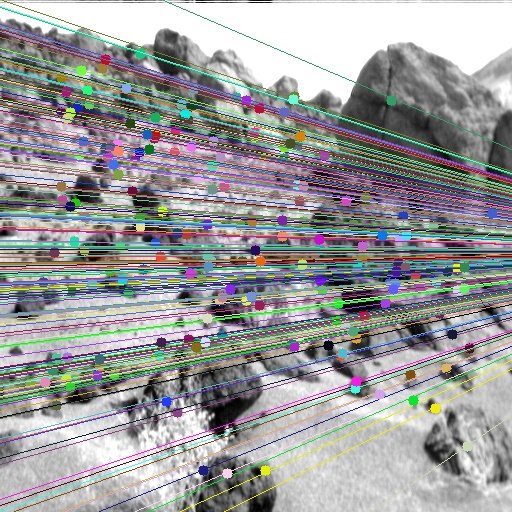
\includegraphics[width=0.5\textwidth]{img13}
            \label{img13}
        }
        \subfigure[Imagen vmort2 con las líneas epipolares pintadas]{
            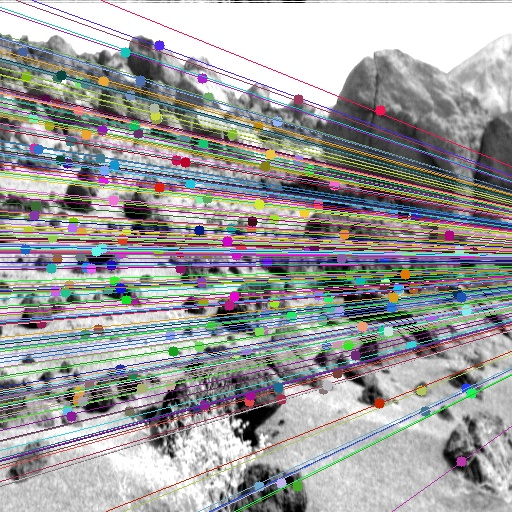
\includegraphics[width=0.5\textwidth]{img14}
            \label{img14}
        }
    }
    \caption{Líneas epipolares sobre ambas imágenes}
    \label{vmort}
\end{figure}

En la \hyperref[vmort]{Figura \ref*{vmort}} vemos el resultado de la función desarrollada. El resultado obtenido es bastante bueno, ya que, a simple vista, los puntos en correspondencias calculados se encuentran sobre su correspondiente línea epipolar.

\subsection{Verificar la bondad de $F$ calculando la media de la distancia ortogonal entre los puntos soporte y sus líneas epipolares en ambas imágenes. Mostrar el error medio.}

Para poder realizar este apartado, he definido varias funciones. En primer lugar, he definido una función para calcular la distancia entre un punto y una recta, basándome en las explicaciones de \cite{wiki}:

\begin{displaymath}
distance(ax + by + c = 0, (x_0, y_0)) = \frac{\left| ax_0 + by_0 + c \right|}{\sqrt{a^2 + b^2}}
\end{displaymath}

Después, he definido una función para calcular la media del cuadrado de la distancia entre cada punto y su correspondiente recta epipolar:

\begin{displaymath}
\sum_i d(x_i, F x_i')^2
\end{displaymath}

Por último, he definido una función para calcular el \textbf{error epipolar simétrico}:

\begin{displaymath}
\sum_i d(x_i, F x_i')^2 + d(x_i', F x_i)^2
\end{displaymath}

\begin{minted}[frame=lines, label={Estimando el error de F}]{python}
def distance_point_line(point, line):
    x0, y0 = point
    a, b, c = line
    return np.abs(a*x0 + b*y0 + c)/np.sqrt(a*a + b*b)

def epipolar_distance_points_lines(points, lines):
    n = points.shape[0]
    distance = np.zeros(n, np.float32)
    for i in range(n):
        d = distance_point_line(point=points[i], line=lines[i][0])
        distance[i] = d
    return np.mean(distance)

def epipolar_symmetric_error(points1, lines1, points2, lines2):
    # calculamos la media de las distancias de cada punto a su línea epipolar
    distance1 = epipolar_distance_points_lines(points=points1, lines=lines1)
    distance2 = epipolar_distance_points_lines(points=points2, lines=lines2)
    # aplicamos la fórmula
    return (distance1 + distance2)/2
\end{minted}

El error de $F$ calculado por esta función fue $1.01102924347$. Como se veía en las líneas epipolares pintadas sobre las imágenes, la estimación de $F$ parecía ser bastante buena. Debido a que tiene un error bastante bajo, podemos confirmar la afirmación que hicimos antes.

\section{Cálculo del movimiento de la cámara ($R$, $t$) asociado a cada pareja de imágenes calibradas.}

\subsection{Leer las imágenes y los datos de calibración.}

En este apartado, disponemos de una serie de imágenes denominadas \textit{reconstruccion/rdimage.00x.ppm}, donde $x$ representa el número de imagen. Cada imagen viene acompañada de un fichero de igual nombre y terminación \textit{.camera}. 

\begin{minted}[frame=lines, label={Leyendo las imágenes y sus parámetros}]{python}
def read_images_and_calibration_parameters(img, calib_file):
    # en primer lugar leemos la imagen y, después, los parámetros de rotación y
    # traslación que tiene asociados
    img_m = cv2.imread(filename=img)
    rotacion = np.zeros(shape=(3,3), dtype=np.float32)
    traslacion = np.zeros(shape=(3), dtype=np.float32)
    camera = np.zeros(shape=(3,3), dtype=np.float32)
    with open(calib_file) as f:
        lines = f.readlines()
    traslacion = np.array(lines[7].split(sep=" ")[:3], dtype=np.float32)
    for i in range(3):
        rotacion[i] = np.array(lines[i+4].split(sep=" ")[:3], dtype=np.float32)
        camera[i] = np.array(lines[i].split(sep=" ")[:3], dtype=np.float32)

    return img_m, camera, rotacion, traslacion
\end{minted}

\subsection{Calcular parejas de puntos en correspondencia entre las imágenes.}

Para realizar este apartado, he usado las mismas funciones que en el ejercicio anterior.

\begin{minted}[frame=lines, label={Extrayendo correspondencias}]{python}
matches, kps1, kps2 = get_match(img1=imgs[0], img2=imgs[1], type="BRISK", 
                        mostrar_img=False, knn_matching=False)
\end{minted}

\subsection{Estimar la matriz esencial y calcular el movimiento.}

Para realizar este apartado, me he basado en las explicaciones de \cite{mvg}.

\subsubsection{Estimar la matriz esencial}

La ecuación que define la matriz esencial es:

\begin{displaymath}
\hat{x}'^T E \hat{x} = 0
\end{displaymath}

donde $x$ y $x'$ son puntos en correspondencias, $x \leftrightarrow x'$.  Si sustituimos $\hat{x}$ y $\hat{x}'$ obtenemos:

\begin{displaymath}
x'^T K'^{-T} E K^{-1} x = 0
\end{displaymath}

comparando esta ecuación con la ecuación de la matriz fundamental, $x'Fx = 0$, finalmente concluimos que podemos calcular la matriz esencial como:

\begin{displaymath}
E = K'^T F K
\end{displaymath}

\begin{minted}[frame=lines, label={Estimando E}]{python}
def my_find_essential_matrix(F, camera):
    # la matriz cámara es igual para ambas imágenes
    E = camera[1].T.dot(F.dot(camera[0]))
    print("Matriz esencial")
    print(E)
    return E
\end{minted}

La matriz esencial obtenida fue:

\begin{displaymath}
\left[
\begin{matrix}
0.42470622 & -250.02808332 & -58.88594738 \\
247.55404323 &   32.66746787 &  44.56350471 \\
57.03102359 &  -30.54830715 &   1.30896057 
\end{matrix}
\right]
\end{displaymath}

Una matriz $3 \times 3$ es una matriz esencial sí y solo sí dos de sus valores singulares son iguales y el tercero es igual a cero. En el caso de la matriz esencial obtenida, sus autovalores fueron:

\begin{displaymath}
\left[
\begin{matrix}
276.182556 & 241.305817  & 5.17288716 \cdot 10^{-12}\\
\end{matrix}
\right]
\end{displaymath}

En este caso, dos de los valores singulares que hemos obtenido son muy parecidos entre sí ($276.18$ y $241.3$) y el último es muy cercano a cero, por lo que podemos considerar que la matriz obtenida cumple la condición para ser una matriz esencial.

\subsubsection{Calcular el movimiento}

En primer lugar, debemos definir la matriz $W$:

\begin{displaymath}
W = \left[ \begin{matrix}
0 & -1 & 0 \\
1 & 0 & 0 \\
0 & 0 & 1
\end{matrix} \right] 
\end{displaymath}

Suponiendo que la descomposición en valores singulares de $E$ es:

\begin{displaymath}
U diag(1,1,0) V^T
\end{displaymath}

podemos obtener dos $R$ distintos:

\begin{displaymath}
R = UWV^T \qquad\ R = UW^T V^T
\end{displaymath}

La traslación se calcula como:

\begin{displaymath}
t = U(0,0,1)^T = u_3
\end{displaymath}

es decir, la última columna de $U$. El signo de $E$, y por tanto el signo de $t$, es desconocido.

Por tanto, dada una matriz esencial $E = U diag(1,1,0) V^T$ y una primera matriz cámara $P = [I | 0]$, hay cuatro posibles soluciones para la segunda cámara $P'$:

\begin{displaymath}
P' = [UWV^T | \;u_3] \qquad\ P' = [UWV^T | -u_3] \qquad\ P' = [UW^T V^T |\; u_3] \qquad\ P' = [UW^T V^T | -u_3]
\end{displaymath}

La diferencia entre las dos primeras es la dirección, dada por $t$; en cambio, la diferencia entre la primera y la tercera  es que esta última está girada $180^{\circ}$ con respecto de la primera. 

La cámara que nosotros elegiremos debe tener todos los puntos delante de la cámara, es decir, con profundidad positiva. Ya que una cámara no puede fotografiar puntos que queden detrás suya. Para saber esto, haremos una triangulación 3D de los puntos en correspondencias obtenidos.

\begin{minted}[frame=lines, label={Calculando los R y T}]{python}
def compute_r_and_t(E):
    # descomponemos E en valores singulares. D = diag(1,1,0)^T
    U,D,V = np.linalg.svd(a=E)
    W = np.array([[0,-1,0],[1,0,0],[0,0,1]])
    # puede hacer dos Rs distintas: R = UWV^T o UW^TV^T
    R_1 = U.dot(W.dot(V.T))
    R_2 = U.dot(W.T.dot(V.T))
    # y puede haber dos T distintas -u3 o u3:
    T_1 = U[:,2]
    T_2 = -U[:,2]
    return R_1, R_2, T_1, T_2
\end{minted}

Para calcular la triangulación 3D de un punto ($X$), partimos de las ecuaciones de los puntos en correspondencias que tenemos: 

\begin{displaymath}
x = PX \qquad\ x' = P'X
\end{displaymath}

Estas ecuaciones pueden combinarse de la forma $AX = 0$, es decir, una ecuación lineal en $X$:

\begin{displaymath}
A = \left[ \begin{matrix}
x p^{3T} - p^{1T} \\
y p^{3T} - p^{2T} \\
x' p'^{3T} - p'^{1T} \\
y' p'^{3T} - p'^{2T}
\end{matrix} \right]
\end{displaymath}

donde $p^{iT}$ es la $i$-ésima fila de $P$.

Resolvemos esta ecuación para cada par de puntos en correspondencias, obteniendo así sus correspondientes coordenadas 3D. Hacemos esto para cada solución obtenida y comprobamos cuál obtiene un menor número de puntos negativos.

\begin{minted}[frame=lines, label={Estimando la cámara correcta}]{python}
def triangulation(P, P1, point1, point2):
    # renombramos los puntos a x, y, x' e y'.
    x, y = point1[0], point1[1]
    x1, y1 = point2[0], point2[1]
    # construimos la matriz A
    A = np.zeros(shape=(4,4), dtype=np.float32)
    A[0] = x*P[2] - P[0]
    A[1] = y*P[2] - P[1]
    A[2] = x1*P1[2] - P1[0]
    A[3] = y1*P1[2] - P1[1]
    # una vez tenemos A, calculamos su descomposición en valores singulares
    U, W, V = np.linalg.svd(a=A)
    return V[3]/V[3,-1]

# función que, a partir de K, R y T crea una matriz cámara
def camera_matrix(K, R, T):
    T = T.reshape(1,3)
    cmatrix = np.hstack((R,T.T))
    return K.dot(cmatrix)

def test_if_point_is_in_front(K, R_1, R_2, T_1, T_2, pts1, pts2):
    # construimos las cuatro posibles soluciones
    camera1 = camera_matrix(K=K[1], R=R_1, T=T_1)
    camera2 = camera_matrix(K=K[1], R=R_1, T=T_2)
    camera3 = camera_matrix(K=K[1], R=R_2, T=T_1)
    camera4 = camera_matrix(K=K[1], R=R_2, T=T_2)
    # y la cámara identidad
    camera0 = K[0].dot(np.array([[1,0,0,0],[0,1,0,0],[0,0,1,0]]))
    # calculamos los puntos 3D con las cuatro soluciones
    sols = []
    for cam in [camera1, camera2, camera3, camera4]:
        sol = []
        for pt1, pt2 in zip(pts1, pts2):
            X = triangulation(P=camera0, P1=cam, point1=pt1, point2=pt2)
            sol.append(X)
        sol = np.array(sol)
        sols.append(np.where(sol[:,2] < 0)[0].size)

    print("Número de puntos negativos encontrados por cada cámara")
    print(sols)

    return [(R_1,T_1),(R_1,T_2),(R_2,T_1),(R_2,T_2)][min(sols)]
\end{minted}

El número de puntos negativos encontrados por cada cámara fue:

\begin{enumerate}[---]
    \item $[UWV^T | \;u_3]$: $0$
    \item $[UWV^T | -u_3]$: $2201$
    \item $[UW^T V^T |\; u_3]$: $189$
    \item $[UW^T V^T | -u_3]$: $2012$
\end{enumerate}

La cámara correcta es aquella con la que ningún punto ha sido negativo, es decir, la primera cámara.

\bibliography{bibliografia} %archivo citas.bib que contiene las entradas 
\bibliographystyle{siam} % hay varias formas de citar

\end{document}